% ============================================================
%  Section 10 – Future Research Directions
% ============================================================
\section{Future Research Directions}
\label{sec:future}

The limitations identified in Section~\ref{sec:limitations} define the
boundaries of the current \uvif{} contribution and, simultaneously, the
agenda for its further development. We outline five research directions
that we consider most pressing.

\begin{figure}[!t]
\centering
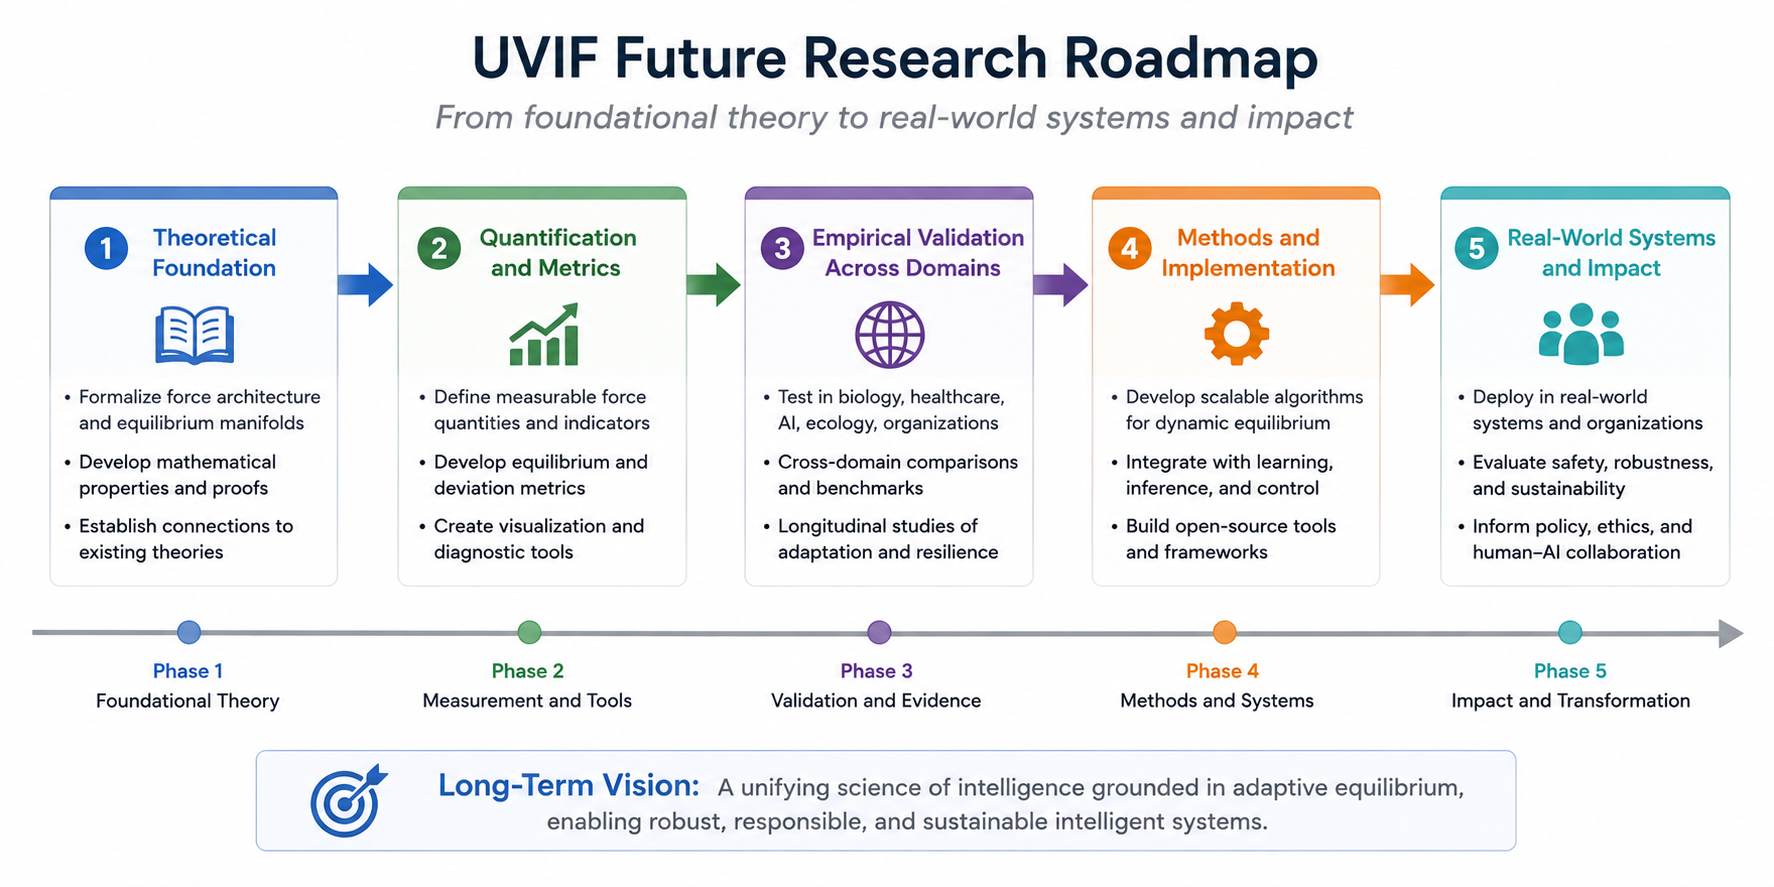
\includegraphics[width=\linewidth]{Figures/Fig10_Future_Roadmap.png}
\caption{UVIF future research roadmap. The framework evolves through
five major stages: theoretical formalization, equilibrium quantification,
cross-domain empirical validation, scalable implementation, and
real-world deployment. The long-term objective is the development of a
unified science of intelligence grounded in adaptive equilibrium,
bounded knowledge, sustainability, and persistent viability.}
\label{fig:future_roadmap}
\end{figure}

Fig.~\ref{fig:future_roadmap} presents a structured roadmap for the
future development of \uvif{}. The figure emphasizes that the framework
should not remain only a conceptual philosophy of intelligence. Rather,
it should progressively evolve into a mathematically grounded,
empirically validated, and operationally deployable scientific
framework.

The first stage concerns \emph{theoretical foundation}. Future work
must formalize the geometry of Variational Equilibrium manifolds,
rigorously define force interactions, establish stability properties,
and connect \uvif{} with existing mathematical theories of dynamical
systems, variational flows, stochastic processes, and viability
analysis.

The second stage focuses on \emph{quantification and metrics}. The
framework will require measurable quantities capable of estimating force
balance, equilibrium proximity, system deviation, adaptive resilience,
and sustainability under changing conditions. These metrics will be
necessary for transforming \uvif{} from a qualitative framework into a
testable scientific methodology.

The third stage involves \emph{empirical validation across domains}.
One of the defining characteristics of \uvif{} is its cross-domain
scope. Consequently, future research must evaluate the framework across
biology, healthcare, artificial intelligence, ecology, cognition, and
organizational systems in order to determine whether the proposed
organizational principles consistently emerge in real-world adaptive
systems.

The fourth stage concerns \emph{methods and implementation}. This stage
includes the development of scalable algorithms, equilibrium-aware AI
architectures, adaptive control mechanisms, uncertainty-aware decision
systems, and computationally sustainable intelligent systems capable of
maintaining dynamic equilibrium under partial observability and noisy
environments.

The fifth stage represents \emph{real-world systems and impact}. The
long-term vision of \uvif{} is not merely theoretical elegance, but the
development of safer, more sustainable, more resilient, and more
human-compatible intelligent systems capable of operating coherently
under uncertainty, changing environments, and long temporal horizons.

The roadmap shown in the figure also reinforces an important conceptual
point of this paper: the development of intelligence research may
require a transition away from isolated short-term optimization and
toward adaptive equilibrium, bounded knowability, sustainability, and
persistent viability as central organizational principles.

\subsection{PDE-Based Variational Dynamics}

The most natural mathematical language for \uvif{} in spatially
extended systems is that of partial differential equations (PDEs).
Many of the systems to which \uvif{} applies---ecosystems, neural
fields, social networks---have structure in space as well as time,
and the Variational Equilibrium of such systems is a spatial pattern,
not just a single configuration.

The mathematical theory of variational methods for evolution---
encompassing gradient flows, free energy functionals, and metric-space
geometry \citep{campos2021discrete}---provides the starting point
for this development. The challenge is to formulate the five forces
of \uvif{} as terms in a PDE system in a way that is both
mathematically tractable and phenomenologically faithful to the
systems being modeled.

A promising approach is to formulate the force dynamics as a
gradient flow on a suitable state space, where the energy functional
captures the five forces and the Variational Equilibrium is the
minimizer of this functional. Existence and regularity of solutions
can then be studied using tools from the theory of evolution equations
in Banach and Hilbert spaces. The connection to the variational methods
for ecosystem dynamics studied in ecology \citep{kefi2024selforg,
rietkerk2021evasion} and the free-energy dynamics studied in
neuroscience \citep{friston2010fep,kim2022freeenergy} will be
particularly fruitful.

\subsection{Nature-Inspired Adaptive AI Architectures}

The second research direction is the engineering of AI architectures
that explicitly instantiate the \uvif{} force balance. Current
architectures---transformers, convolutional networks, recurrent
networks---are designed around the efficient implementation of
specific computational operations, not around the maintenance of
a force balance. Building \uvif{}-aligned architectures requires
rethinking the structure of learning systems from the ground up.

Promising directions include:
\begin{itemize}[leftmargin=1.5em]
  \item \emph{Modular architectures} that separate the components
    responsible for epistemic pull (active learning, uncertainty
    estimation), selective protection (knowledge consolidation, memory
    replay), computational efficiency (pruning, sparse computation),
    and sustainability (resource monitoring, adaptive computation).
  \item \emph{Intrinsic motivation mechanisms} that implement the
    epistemic pull force as an endogenous reward for information gain,
    integrated with extrinsic task performance signals
    \citep{friston2017curiosity,dubey2019curiosity}.
  \item \emph{Biomimetic regularization} schemes that implement
    selective protection by drawing on the biological principles of
    synaptic consolidation, replay, and homeostatic plasticity
    \citep{moreddu2025bioinspired,diaz2025biomimetics}.
\end{itemize}

The green AI literature provides an important constraint: the
architectures developed should be evaluated not only for their
performance but for their energy efficiency and computational
sustainability \citep{bolon2024greenai}. A \uvif{}-aligned architecture
that requires massive computational resources to maintain its force
balance has failed to instantiate the computational drag force
adequately.

\subsection{Multi-Agent Equilibrium Systems}

The third research direction extends \uvif{} from single-agent to
multi-agent systems. When multiple \uvif{}-aligned agents interact,
the system-level Variational Equilibrium is not simply the sum of
the individual agents' equilibria; it is a collective configuration
that emerges from the interactions between agents, each pursuing its
own force balance.

The natural theoretical framework for this extension is
game theory. Multi-agent Nash equilibria \citep{semsar2009multiagent,
wang2022cooperative} provide the micro-level mechanism by which
macro-level Variational Equilibria are generated in multi-agent
systems. The challenge is to design individual agent force architectures
such that the resulting Nash equilibria are close to the socially
optimal Variational Equilibrium---the configuration that maximizes
the collective force balance \citep{memarzadeh2020food}.

This is a multi-agent analog of the alignment problem in AI safety:
how can individually rational agents be designed so that their
collective behavior is beneficial? The \uvif{} framework suggests that
the answer lies in giving each agent a sustainability force that is
sensitive to the collective system's resource use, so that individual
agents are naturally incentivized to avoid behaviors that deplete the
shared environment.

Ecological models of co-evolutionary dynamics---where organisms evolve
strategies that are individually adaptive and collectively sustainable
---provide empirical inspiration for this research direction
\citep{levin1998ecosystems,dyke2013environmental}. The theoretical
tools of evolutionary game theory, mean-field games, and cooperative
game theory will all be relevant.

\subsection{Sustainable and Self-Regulating Intelligence}

The fourth research direction is the development of AI systems that
actively maintain their own Variational Equilibrium---systems that
are not only designed with the force balance in mind but that monitor
their own operating configuration and take corrective action when
displaced from equilibrium.

This is the AI analog of biological self-regulation: the capacity
of a living system to detect deviations from homeostatic set-points
and deploy corrective responses. In artificial systems, it requires:
\begin{itemize}[leftmargin=1.5em]
  \item \emph{Force monitoring}: mechanisms that estimate the current
    values of the five forces from observable system behavior.
  \item \emph{Equilibrium detection}: methods for determining whether
    the current state is within the basin of attraction of the
    Variational Equilibrium.
  \item \emph{Corrective dynamics}: algorithms that, upon detecting
    displacement from equilibrium, modulate the system's behavior
    to restore the force balance.
\end{itemize}

The free-energy principle's account of allostasis---the active
adjustment of set-points in response to anticipated perturbations
---provides a starting point for the third component
\citep{bettinger2023physiological,kim2022freeenergy}. Adaptive
homeostasis in biology, where the homeostatic range expands or
contracts in response to sub-threshold stimuli, provides a model
for how set-point adaptation can be incorporated into the \uvif{}
dynamics \citep{davies2016adaptive}.

\subsection{Toward Unified Organizational Theories of Intelligence}

The fifth research direction is the most ambitious: the development
of a genuinely unified theory of intelligence that subsumes the
biological, ecological, cognitive, artificial, and organizational
domains within a single formal framework.

Such a theory would need to:
\begin{itemize}[leftmargin=1.5em]
  \item Provide formal definitions of the five \uvif{} forces that
    are applicable across all domains, together with domain-specific
    instantiations.
  \item Derive quantitative predictions about the relationship between
    force balance and system performance (intelligence, health,
    resilience, sustainability) in each domain.
  \item Show that existing domain-specific theories
    (homeostasis, ecological resilience, free-energy principle,
    organizational learning) are special cases of or can be embedded
    within the \uvif{} framework.
  \item Identify universal signatures of Variational Equilibrium
    that can be observed across domains---metrics that indicate
    proximity to equilibrium regardless of the specific system
    being studied.
\end{itemize}

The unification of theories that have developed in relative isolation
is one of the most challenging and most productive activities in
science. The history of science offers many examples---statistical
mechanics unifying thermodynamics and atomic theory; the modern
synthesis unifying genetics and evolution; quantum electrodynamics
unifying quantum mechanics and electromagnetism---of unifications
that transformed entire fields. The \uvif{} framework is proposed
in this spirit: as a candidate for the unifying framework that the
science of intelligence---biological, artificial, and organizational---
currently lacks.



% Deep revision placeholder inserted.
% [Further conceptual integration recommended]
